% Options for packages loaded elsewhere
\PassOptionsToPackage{unicode}{hyperref}
\PassOptionsToPackage{hyphens}{url}
\PassOptionsToPackage{dvipsnames,svgnames,x11names}{xcolor}
%
\documentclass[
  letterpaper,
  DIV=11,
  numbers=noendperiod]{scrartcl}

\usepackage{amsmath,amssymb}
\usepackage{lmodern}
\usepackage{iftex}
\ifPDFTeX
  \usepackage[T1]{fontenc}
  \usepackage[utf8]{inputenc}
  \usepackage{textcomp} % provide euro and other symbols
\else % if luatex or xetex
  \usepackage{unicode-math}
  \defaultfontfeatures{Scale=MatchLowercase}
  \defaultfontfeatures[\rmfamily]{Ligatures=TeX,Scale=1}
\fi
% Use upquote if available, for straight quotes in verbatim environments
\IfFileExists{upquote.sty}{\usepackage{upquote}}{}
\IfFileExists{microtype.sty}{% use microtype if available
  \usepackage[]{microtype}
  \UseMicrotypeSet[protrusion]{basicmath} % disable protrusion for tt fonts
}{}
\makeatletter
\@ifundefined{KOMAClassName}{% if non-KOMA class
  \IfFileExists{parskip.sty}{%
    \usepackage{parskip}
  }{% else
    \setlength{\parindent}{0pt}
    \setlength{\parskip}{6pt plus 2pt minus 1pt}}
}{% if KOMA class
  \KOMAoptions{parskip=half}}
\makeatother
\usepackage{xcolor}
\setlength{\emergencystretch}{3em} % prevent overfull lines
\setcounter{secnumdepth}{-\maxdimen} % remove section numbering
% Make \paragraph and \subparagraph free-standing
\ifx\paragraph\undefined\else
  \let\oldparagraph\paragraph
  \renewcommand{\paragraph}[1]{\oldparagraph{#1}\mbox{}}
\fi
\ifx\subparagraph\undefined\else
  \let\oldsubparagraph\subparagraph
  \renewcommand{\subparagraph}[1]{\oldsubparagraph{#1}\mbox{}}
\fi

\usepackage{color}
\usepackage{fancyvrb}
\newcommand{\VerbBar}{|}
\newcommand{\VERB}{\Verb[commandchars=\\\{\}]}
\DefineVerbatimEnvironment{Highlighting}{Verbatim}{commandchars=\\\{\}}
% Add ',fontsize=\small' for more characters per line
\usepackage{framed}
\definecolor{shadecolor}{RGB}{241,243,245}
\newenvironment{Shaded}{\begin{snugshade}}{\end{snugshade}}
\newcommand{\AlertTok}[1]{\textcolor[rgb]{0.68,0.00,0.00}{#1}}
\newcommand{\AnnotationTok}[1]{\textcolor[rgb]{0.37,0.37,0.37}{#1}}
\newcommand{\AttributeTok}[1]{\textcolor[rgb]{0.40,0.45,0.13}{#1}}
\newcommand{\BaseNTok}[1]{\textcolor[rgb]{0.68,0.00,0.00}{#1}}
\newcommand{\BuiltInTok}[1]{\textcolor[rgb]{0.00,0.23,0.31}{#1}}
\newcommand{\CharTok}[1]{\textcolor[rgb]{0.13,0.47,0.30}{#1}}
\newcommand{\CommentTok}[1]{\textcolor[rgb]{0.37,0.37,0.37}{#1}}
\newcommand{\CommentVarTok}[1]{\textcolor[rgb]{0.37,0.37,0.37}{\textit{#1}}}
\newcommand{\ConstantTok}[1]{\textcolor[rgb]{0.56,0.35,0.01}{#1}}
\newcommand{\ControlFlowTok}[1]{\textcolor[rgb]{0.00,0.23,0.31}{#1}}
\newcommand{\DataTypeTok}[1]{\textcolor[rgb]{0.68,0.00,0.00}{#1}}
\newcommand{\DecValTok}[1]{\textcolor[rgb]{0.68,0.00,0.00}{#1}}
\newcommand{\DocumentationTok}[1]{\textcolor[rgb]{0.37,0.37,0.37}{\textit{#1}}}
\newcommand{\ErrorTok}[1]{\textcolor[rgb]{0.68,0.00,0.00}{#1}}
\newcommand{\ExtensionTok}[1]{\textcolor[rgb]{0.00,0.23,0.31}{#1}}
\newcommand{\FloatTok}[1]{\textcolor[rgb]{0.68,0.00,0.00}{#1}}
\newcommand{\FunctionTok}[1]{\textcolor[rgb]{0.28,0.35,0.67}{#1}}
\newcommand{\ImportTok}[1]{\textcolor[rgb]{0.00,0.46,0.62}{#1}}
\newcommand{\InformationTok}[1]{\textcolor[rgb]{0.37,0.37,0.37}{#1}}
\newcommand{\KeywordTok}[1]{\textcolor[rgb]{0.00,0.23,0.31}{#1}}
\newcommand{\NormalTok}[1]{\textcolor[rgb]{0.00,0.23,0.31}{#1}}
\newcommand{\OperatorTok}[1]{\textcolor[rgb]{0.37,0.37,0.37}{#1}}
\newcommand{\OtherTok}[1]{\textcolor[rgb]{0.00,0.23,0.31}{#1}}
\newcommand{\PreprocessorTok}[1]{\textcolor[rgb]{0.68,0.00,0.00}{#1}}
\newcommand{\RegionMarkerTok}[1]{\textcolor[rgb]{0.00,0.23,0.31}{#1}}
\newcommand{\SpecialCharTok}[1]{\textcolor[rgb]{0.37,0.37,0.37}{#1}}
\newcommand{\SpecialStringTok}[1]{\textcolor[rgb]{0.13,0.47,0.30}{#1}}
\newcommand{\StringTok}[1]{\textcolor[rgb]{0.13,0.47,0.30}{#1}}
\newcommand{\VariableTok}[1]{\textcolor[rgb]{0.07,0.07,0.07}{#1}}
\newcommand{\VerbatimStringTok}[1]{\textcolor[rgb]{0.13,0.47,0.30}{#1}}
\newcommand{\WarningTok}[1]{\textcolor[rgb]{0.37,0.37,0.37}{\textit{#1}}}

\providecommand{\tightlist}{%
  \setlength{\itemsep}{0pt}\setlength{\parskip}{0pt}}\usepackage{longtable,booktabs,array}
\usepackage{calc} % for calculating minipage widths
% Correct order of tables after \paragraph or \subparagraph
\usepackage{etoolbox}
\makeatletter
\patchcmd\longtable{\par}{\if@noskipsec\mbox{}\fi\par}{}{}
\makeatother
% Allow footnotes in longtable head/foot
\IfFileExists{footnotehyper.sty}{\usepackage{footnotehyper}}{\usepackage{footnote}}
\makesavenoteenv{longtable}
\usepackage{graphicx}
\makeatletter
\def\maxwidth{\ifdim\Gin@nat@width>\linewidth\linewidth\else\Gin@nat@width\fi}
\def\maxheight{\ifdim\Gin@nat@height>\textheight\textheight\else\Gin@nat@height\fi}
\makeatother
% Scale images if necessary, so that they will not overflow the page
% margins by default, and it is still possible to overwrite the defaults
% using explicit options in \includegraphics[width, height, ...]{}
\setkeys{Gin}{width=\maxwidth,height=\maxheight,keepaspectratio}
% Set default figure placement to htbp
\makeatletter
\def\fps@figure{htbp}
\makeatother

\KOMAoption{captions}{tableheading}
\makeatletter
\makeatother
\makeatletter
\makeatother
\makeatletter
\@ifpackageloaded{caption}{}{\usepackage{caption}}
\AtBeginDocument{%
\ifdefined\contentsname
  \renewcommand*\contentsname{Table of contents}
\else
  \newcommand\contentsname{Table of contents}
\fi
\ifdefined\listfigurename
  \renewcommand*\listfigurename{List of Figures}
\else
  \newcommand\listfigurename{List of Figures}
\fi
\ifdefined\listtablename
  \renewcommand*\listtablename{List of Tables}
\else
  \newcommand\listtablename{List of Tables}
\fi
\ifdefined\figurename
  \renewcommand*\figurename{Figure}
\else
  \newcommand\figurename{Figure}
\fi
\ifdefined\tablename
  \renewcommand*\tablename{Table}
\else
  \newcommand\tablename{Table}
\fi
}
\@ifpackageloaded{float}{}{\usepackage{float}}
\floatstyle{ruled}
\@ifundefined{c@chapter}{\newfloat{codelisting}{h}{lop}}{\newfloat{codelisting}{h}{lop}[chapter]}
\floatname{codelisting}{Listing}
\newcommand*\listoflistings{\listof{codelisting}{List of Listings}}
\makeatother
\makeatletter
\@ifpackageloaded{caption}{}{\usepackage{caption}}
\@ifpackageloaded{subcaption}{}{\usepackage{subcaption}}
\makeatother
\makeatletter
\@ifpackageloaded{tcolorbox}{}{\usepackage[many]{tcolorbox}}
\makeatother
\makeatletter
\@ifundefined{shadecolor}{\definecolor{shadecolor}{rgb}{.97, .97, .97}}
\makeatother
\makeatletter
\makeatother
\ifLuaTeX
  \usepackage{selnolig}  % disable illegal ligatures
\fi
\IfFileExists{bookmark.sty}{\usepackage{bookmark}}{\usepackage{hyperref}}
\IfFileExists{xurl.sty}{\usepackage{xurl}}{} % add URL line breaks if available
\urlstyle{same} % disable monospaced font for URLs
\hypersetup{
  pdftitle={Parsons' Paper Company Workers Database},
  pdfauthor={Lorraine Oloo and Camden Heafitz},
  colorlinks=true,
  linkcolor={blue},
  filecolor={Maroon},
  citecolor={Blue},
  urlcolor={Blue},
  pdfcreator={LaTeX via pandoc}}

\title{Parsons' Paper Company Workers Database}
\author{Lorraine Oloo and Camden Heafitz}
\date{2023-02-17}

\begin{document}
\maketitle
\ifdefined\Shaded\renewenvironment{Shaded}{\begin{tcolorbox}[frame hidden, breakable, borderline west={3pt}{0pt}{shadecolor}, enhanced, sharp corners, interior hidden, boxrule=0pt]}{\end{tcolorbox}}\fi

\hypertarget{introduction}{%
\subsection{Introduction}\label{introduction}}

Mining the History of Holyoke (STAT210) is a class at Amherst College
with a mission statement of curating and publishing a piece of Holyoke's
history and making it accessible to the town's people.

One way our class has begun this journey is by analyzing an old payroll
registry found in an attic in Holyoke and now available in the archives
of the Holyoke Public Library History Room. This register tracked pay
for employees who worked at the Parsons Paper Mill in Holyoke,
Massachusetts (the ``Paper City'') in the 1860s.

It has been remarkable to track down so much history as each page of
this nearly 400 page registry has upwards of 30 names, and each name has
its own story worth telling.

In the registry, we can see one's name, number of days worked, their
wages, whether or not the worker had rent or board due, the final
balance owed, and signature (see Figure~\ref{fig-sample}). See
\href{https://r.amherst.edu/apps/nhorton/Parsons-Paper/}{here} for an
interactive display of the register.

\hypertarget{workers-summary}{%
\subsection{Workers' Summary}\label{workers-summary}}

We took on the task of finding information about some of the employees
at the paper mill using the database Ancestry.com.

On page 259, we found two women with the same last name which was common
back then but still we decided to search for one of them on
Ancestry.com.

Their names were Lucy and E.A. Allen. When we searched for Lucy, we
found that E.A. stood for Eliza Ann Allen--they were sisters! (see
Figure~\ref{fig-sample4})

Lucy was born in Massachusetts in 1842 and Eliza Ann was her older
sister born in 1841. They lived in dwelling 42.

Their father's name was Job Allen and their mother was Anna Allen.

Job was born in England and moved to the United States sometime before
1841.

Like his daughters, he too worked at the Parsons Paper Company.

We found record of him first on page 3. (see Figure~\ref{fig-sample7})

Anna Allen stayed at home.

This was a common life for a working-class family in Holyoke,
Massachusetts in the 1860s.

From what we were able to gather, Eliza and Lucy were finishers meaning
they helped with finalizing the paper making process.

We made this assumption when we found Lucy's name on Page 2 under the
label ``Finishers.''

See (Figure~\ref{fig-sample9})

Eliza and Lucy were paid not by the number of hours or days they worked
but rather the number of reams they finished.

We can see on page on page 2 that Lucy finished 756 reams of paper for
the month of January in 1861.

Eliza's name first appeared in 1862 on page 34 right below her sisters
name, one year after her sister first started working. (see
Figure~\ref{fig-sample10})

Coincidentally, they were one year apart in age.

Perhaps their father Job did not want his daughters to work until they
were 20 years of age.

It seemed that the Allen family had trouble finding a permanent
residence as we found a number of addresses reported across different
resources.

In 1869, the Holyoke city directory shows that the Allen family lived on
Dwight Street.

Ancestry.com showed that the Allen family lived in dwelling 42 with no
street name reported in 1870.

(see Figure~\ref{fig-sample5})

We were able to follow Lucy's places of residence in several years after
1870 until her death on May 11, 1893 in Holyoke, MA. Here is a
\textbf{map} that shows Lucy's places of residence.

It is also worth noting that Lucy, Eliza, and Job worked for roughly the
entire decade at the mill suggesting the daughters were not pursuing any
form of education in this period. Lucy also appears to have continued
working in the PPC mill until her death.

It is difficult to determine if the Allen family's literacy due to
inconsistencies in signatures.

Some signatures have ``X'' in them while others do not, and the
handwriting is different across the decade suggesting they multiple
people could have been signing for them.

\newpage{}

Conversely, we were able to find records on Joseph C. Parsons; the
founder of the Parsons Paper Company.

(see Figure~\ref{fig-sample8})

Born on February 6, 1814, in Northampton, Hampshire County,
Massachusetts to Lydia and Justice Parsons, Joseph Clark Parsons was a
local businessman who became very successful after founding his mill.

He married Lucretia Hoyt Parsons and had three daughters; Catherine
Turner Taft, Fannie Colton Parsons, and Elizabeth Hoyt Parsons.

We found that Parsons lived in house 22 of dwelling 165 on Suffolk
street which was quite close to his Mill.

This was surprising because we expected him to live in the upper-class
district because wealthier people lived in hills above sea level.~

If we continued our research, we would aim to find descendants of the
Parsons Paper Company that are still living today.

\newpage{}

\hypertarget{technical-appendix}{%
\subsection{\texorpdfstring{\textbf{Technical
Appendix}}{Technical Appendix}}\label{technical-appendix}}

First, we accessed the Amherst College Library account for Ancestry.com.

\begin{figure}

{\centering \includegraphics[width=9.51in,height=0.3\textheight]{amherst_website.png}

}

\caption{\label{fig-sample1}Once on the Amherst website, we clicked the
link to Ancestry Library Edition}

\end{figure}

The link to Amherst's access to ancestry website is
\href{https://libguides.amherst.edu/c.php?g=944984\&p=6812570}{here}.

Here is how the ancestry website looks at a first glance:

\begin{figure}

{\centering \includegraphics[width=9.6in,height=0.325\textheight]{website.jpeg}

}

\caption{\label{fig-sample2}Ancestry.com `search' screen}

\end{figure}

By searching for a name and a place, (Holyoke, Hampden, Massachusetts),
we were able to find census information from the 1800s and track down
paper mill workers.

The number of names that appear in first search. We used educated
guesses to select the most appropriate person.

\begin{figure}

{\centering \includegraphics[width=9.31in,height=0.33\textheight]{multiple_names.jpeg}

}

\caption{\label{fig-sample3}Initial search results}

\end{figure}

The amount of information we could find on each worker varied from name
to name but in general, we were able to find birth year, birthplace,
spouse, children, parents, occupation, and address. Here is what Lucy
and Eliza Ann's profiles looked like on Ancestry.com

\begin{figure}

{\centering \includegraphics[width=0.5\textwidth,height=\textheight]{Lucy_Allen.jpeg}

}

\caption{\label{fig-sample5}Lucy Allen's Profile}

\end{figure}

\begin{figure}

{\centering \includegraphics[width=0.5\textwidth,height=\textheight]{ELIZA_ANN.png}

}

\caption{\label{fig-sample6}Eliza Ann Allen's Profile}

\end{figure}

We then compiled these results into a spreadsheet linked below.

\hypertarget{photo-references}{%
\subsection{Photo References}\label{photo-references}}

\begin{figure}

{\centering \includegraphics[width=9.8in,height=0.47\textheight]{Registry_page_header.jpeg}

}

\caption{\label{fig-sample}Page 259 of the Registry}

\end{figure}

\begin{figure}

{\centering \includegraphics[width=9.36in,height=0.4\textheight]{Joseph_Clark.jpeg}

}

\caption{\label{fig-sample8}Joseph C. Parsons' Profile}

\end{figure}

\begin{figure}

{\centering \includegraphics[width=0.5\textwidth,height=\textheight]{Mary and Eliza Allen.jpeg}

}

\caption{\label{fig-sample4}Lucy and Eliza Ann Allen in the Registry
page 259}

\end{figure}

\begin{figure}

{\centering \includegraphics[width=0.5\textwidth,height=\textheight]{Job Allen page 3 .png}

}

\caption{\label{fig-sample7}Job Allen in the Registry page 3}

\end{figure}

\begin{figure}

{\centering 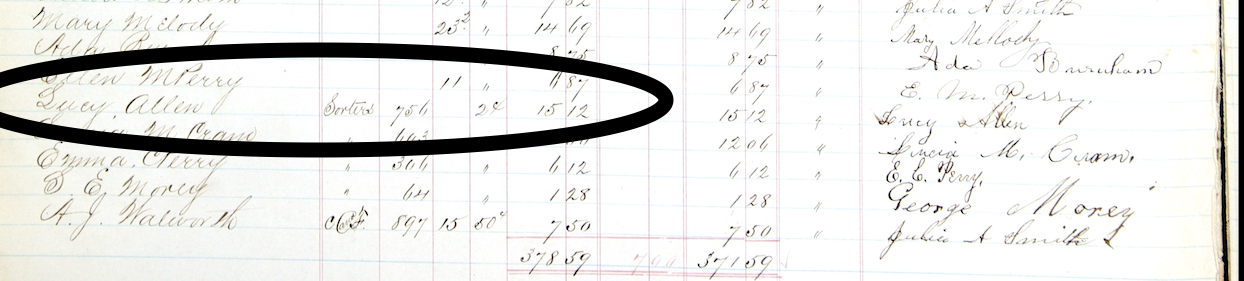
\includegraphics[width=0.6\textwidth,height=\textheight]{Lucypg2.jpeg}

}

\caption{\label{fig-sample9}Lucy Allen in the Registry page 2}

\end{figure}

\begin{figure}

{\centering \includegraphics[width=0.7\textwidth,height=\textheight]{Eliza and lucy allen page 34.png}

}

\caption{\label{fig-sample10}Lucy and Eliza Ann Allen on page 34}

\end{figure}

\hypertarget{map-of-lucy-allens-places-of-residency}{%
\subsection{Map of Lucy Allen's places of
residency}\label{map-of-lucy-allens-places-of-residency}}

\begin{figure}

{\centering \includegraphics[width=0.7\textwidth,height=\textheight]{Lucy Allen map.png}

}

\caption{\label{fig-sample11}Lucy Allen Residency between 1869-91}

\end{figure}

\begin{Shaded}
\begin{Highlighting}[]
\CommentTok{\#library(leaflet)}
\CommentTok{\#m \textless{}{-} leaflet() \%\textgreater{}\%}
  \CommentTok{\#addTiles() \%\textgreater{}\%  \# Add default OpenStreetMap map tiles}
 \CommentTok{\# addMarkers(lng={-}72.610583, lat=42.208699, popup="Lucy\textquotesingle{}s residence in 1869, Dwight Street")\%\textgreater{}\%}
 \CommentTok{\# addMarkers(lng={-}72.60885324421784, lat=42.207205320691806, popup="Lucy\textquotesingle{}s residence in 1883, 236 Maple Street")\%\textgreater{}\%}
 \CommentTok{\# addMarkers(lng={-}72.59690708839962, lat=42.2048726160808, popup="Lucy\textquotesingle{}s residence in 1888{-}1890, rooms 5 Mosher")\%\textgreater{}\%}
  \CommentTok{\# addMarkers(lng={-}72.59879076909023, lat=42.20659749781258, popup="Lucy\textquotesingle{}s residence in 1887 and 1891")\%\textgreater{}\%}
 \CommentTok{\# addMarkers(lng={-}72.61248214421803, lat=42.199421732536955, popup="Parsons Paper Company in the 1800s")}


\CommentTok{\#m  \# Print the map}
\end{Highlighting}
\end{Shaded}

\hypertarget{database}{%
\subsection{Database}\label{database}}

This is the aggregated info for some of the workers who worked in
Parsons' paper in the 1860s:

\begin{Shaded}
\begin{Highlighting}[]
\NormalTok{ancestry }\OtherTok{\textless{}{-}}\NormalTok{ readr}\SpecialCharTok{::}\FunctionTok{read\_csv}\NormalTok{(}\StringTok{"ancestry\_addresses\_updated.csv"}\NormalTok{)}
\end{Highlighting}
\end{Shaded}

\begin{verbatim}
Rows: 22 Columns: 11
-- Column specification --------------------------------------------------------
Delimiter: ","
chr (11): First name, Last Name, Birthday, Death Day, Address, Spouse, Child...

i Use `spec()` to retrieve the full column specification for this data.
i Specify the column types or set `show_col_types = FALSE` to quiet this message.
\end{verbatim}

\begin{Shaded}
\begin{Highlighting}[]
\FunctionTok{glimpse}\NormalTok{(ancestry)}
\end{Highlighting}
\end{Shaded}

\begin{verbatim}
Rows: 22
Columns: 11
$ `First name` <chr> "Ellen", "Joseph", "William", "James", "Patrick", "Patric~
$ `Last Name`  <chr> "Strick", "Parsons", "Kelly", "Casey", "Kelley", "Hollom"~
$ Birthday     <chr> "1859", "2/6/1814", "1834", "1843", "1840", "1835", "1849~
$ `Death Day`  <chr> "N/A", "3/12/1886", "N/A", "N/A", "N/A", "N/A", "N/A", "N~
$ Address      <chr> "N/A", "House 22, Dwelling 165, Suffolk Street", "Holyoke~
$ Spouse       <chr> "N/A", "Lucretia Hoyt Parsons", "Catherine Kelly", "Ann C~
$ Children     <chr> "N/A", "Catherine Turner Taft, Fannie Colton Parsons, Eli~
$ Birthplace   <chr> "Chicopee, Mass", "Northampton, Hampshire County, Massach~
$ Mother       <chr> "N/A", "Lydia Parsons", "Irish", NA, "N/A", "Irish", "Can~
$ Father       <chr> "N/A", "Justice Parsons", "Irish", "Patrick Casey", "N/A"~
$ `US born?`   <chr> "Yes", "Yes", "No", "No", "No", "No", "No", "N/A", "Yes",~
\end{verbatim}

Here is a
\href{https://github.com/STAT210-S23/Parsons_Paper_Register}{LINK} to
this repo



\end{document}
